	\newpage
\section{Ogólne określenie wymagań}		%1
%Ogólne określenie wymagań i zakresu programu (Czyli zleceniodawca określa wymagania programu) 



\hspace{0.60cm}Tutaj może coś być wpisane. 

\subsection{Aplikacja}  %1.1       

\hspace{0.60cm}Aplikacja to PC partpicker w której przez wybranie części komputera przy pozostałych częściach wyświetla się czy są kompatybilne czy nie.

%rysunek
	\begin{figure}[!htb]
	\begin{center}
		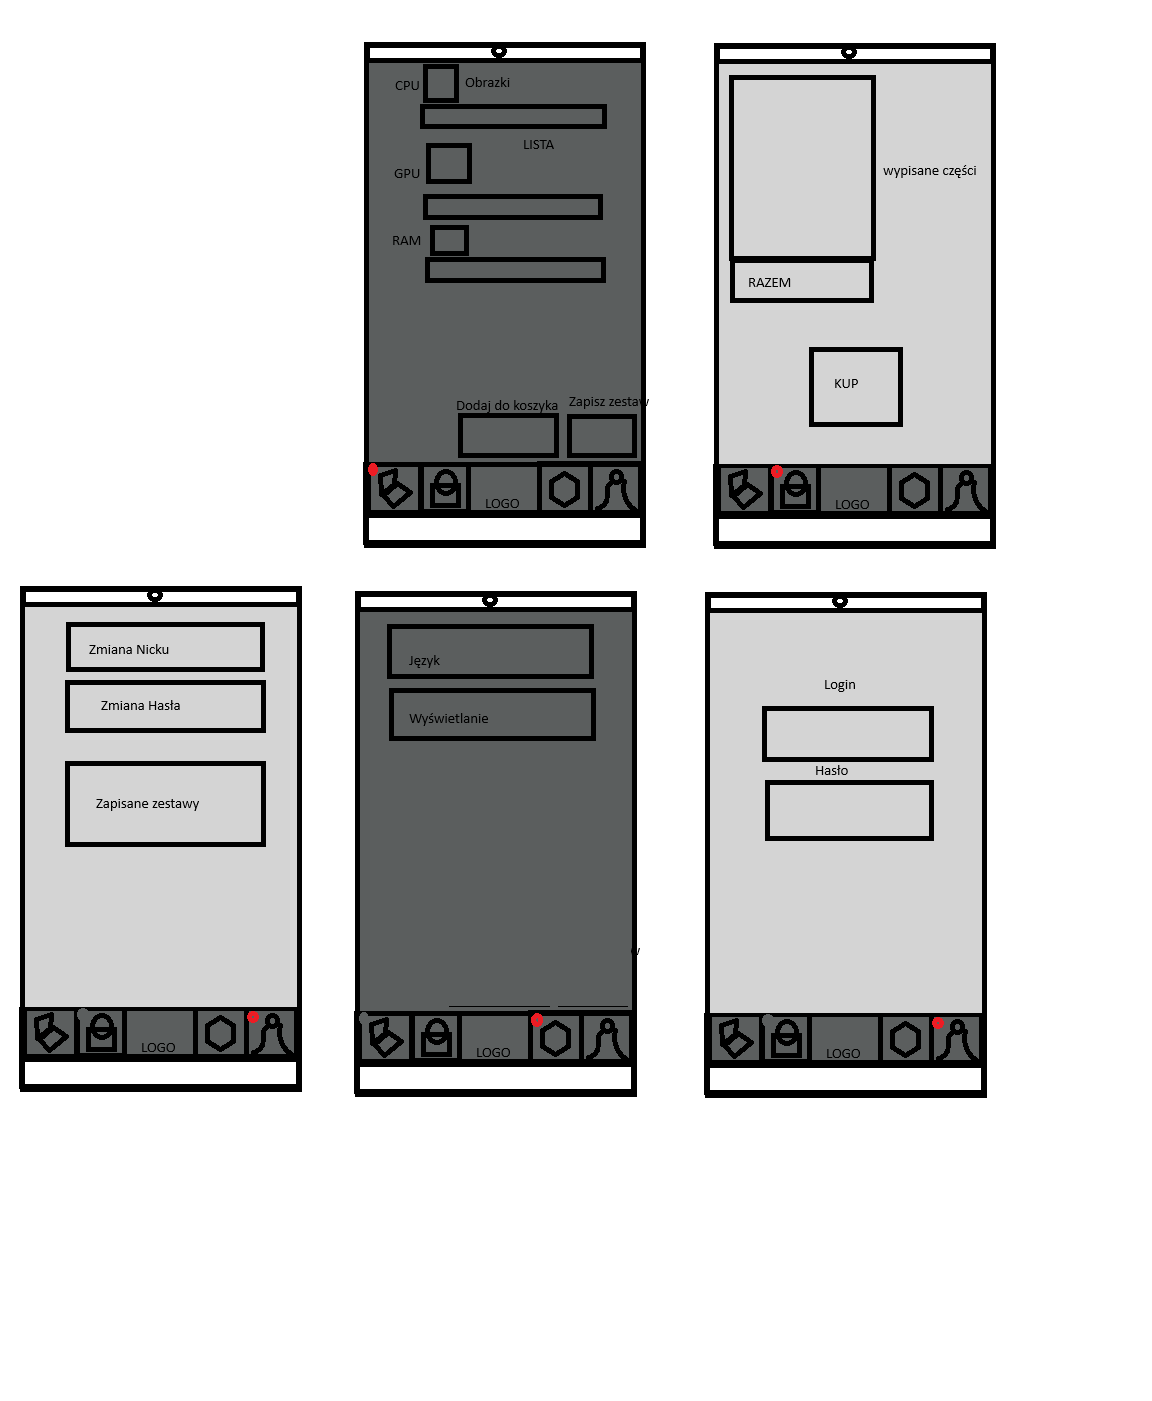
\includegraphics[width=8cm]{rys/wyg.png}
		\caption{wstę☼pny wygląd}
		\label{rys:rysunek001}
	\end{center}
\end{figure}



\subsection{Dodatki}  %1.2

\hspace{0.60cm}Aplikacja ma używać bazy danych firebird.

\begin{figure}[!hbt]
	\begin{center}
		
\includegraphics[width=\linewidth]{rys/bird.jpg}
		\caption{Ustawienie TeXstudio}
		\label{rys:ustawienia}
	\end{center}
\end{figure}
 
 
 
 
 